\documentclass[aspectratio=169]{beamer}

% ---------- fonts & basics ----------
\usepackage[T1]{fontenc}
\usepackage{helvet}
\renewcommand{\familydefault}{\sfdefault}
\usepackage{graphicx}
\usepackage{amsmath,amssymb}

% ---------- tikz ----------
\usepackage{tikz}
\usetikzlibrary{arrows.meta, positioning, calc, shapes.geometric,
                backgrounds, fit, decorations.pathreplacing, shadows}

% ---------- beamer look ----------
\setbeamertemplate{navigation symbols}{}
\setbeamertemplate{footline}{}
\definecolor{navy}{HTML}{1B2A4A}
\definecolor{slategray}{HTML}{5B6B84}
\setbeamercolor{frametitle}{fg=navy,bg=white}
\setbeamerfont{frametitle}{series=\bfseries,size=\large}
\setbeamercolor{normal text}{fg=navy}

% ---------- palette ----------
\definecolor{amber}{HTML}{C8850C}
\definecolor{amberlight}{HTML}{FBF0DA}
\definecolor{skyblue}{HTML}{2E75B6}
\definecolor{skybluelight}{HTML}{E9F2FA}
\definecolor{coral}{HTML}{D4552A}
\definecolor{corallight}{HTML}{FBE9E1}
\definecolor{violet}{HTML}{6449B6}
\definecolor{violetlight}{HTML}{F0ECFA}
\definecolor{ghostgray}{HTML}{C9CFD8}
\definecolor{tealmem}{HTML}{1E7F72}
\definecolor{tealmemlight}{HTML}{E4F3F0}

% ---------- reusable tikz styles ----------
\tikzset{
  >={Latex[length=2.1mm,width=1.5mm]},
  flow/.style={-{Latex[length=2.1mm,width=1.5mm]}, thick, draw=slategray},
  dashedflow/.style={-{Latex[length=1.8mm,width=1.3mm]}, thick, dashed, draw=slategray!70},
  imgcard/.style={draw=slategray!60, thick, rounded corners=1.5pt, fill=white,
                  minimum width=1.15cm, minimum height=1.15cm, inner sep=0pt},
  ghostcard/.style={draw=ghostgray, rounded corners=1.5pt, fill=ghostgray!25,
                     minimum width=1.15cm, minimum height=1.15cm, inner sep=0pt},
  gatebox/.style={rounded corners=3pt, draw=amber, line width=0.9pt, fill=amberlight,
                   align=center, text=navy, font=\scriptsize, text width=2.6cm,
                   minimum height=1.6cm, inner sep=4pt},
  procbox/.style={rounded corners=3pt, draw=coral, line width=0.9pt, fill=corallight,
                   align=center, text=navy, font=\scriptsize, text width=2.4cm,
                   minimum height=1.4cm, inner sep=4pt},
  eqbox/.style={rounded corners=3pt, draw=violet, line width=0.9pt, fill=violetlight,
                   align=center, text=navy, font=\scriptsize, text width=6.4cm,
                   minimum height=1.5cm, inner sep=5pt},
  notebox/.style={rounded corners=3pt, draw=amber!55, line width=0.7pt, fill=amberlight!55,
                   align=center, text=navy, font=\scriptsize, inner sep=5pt},
  bigmem/.style={rounded corners=6pt, draw=violet, line width=1.1pt, fill=violetlight},
  smallcaption/.style={font=\tiny, text=slategray, align=center},
  numcell/.style={draw=slategray!45, thin, minimum width=6.6mm, minimum height=6.2mm,
                   inner sep=0pt, font=\fontsize{5}{5}\selectfont, text=navy},
  % ---- additions for Figures 3-6 ----
  numcellS/.style={draw=slategray!45, thin, minimum width=6.0mm, minimum height=5.4mm,
                   inner sep=0pt, font=\fontsize{4.6}{4.6}\selectfont, text=navy},
  framecard/.style={draw=slategray!70, thick, rounded corners=1.5pt, fill=white, inner sep=0pt},
  cropcard/.style={draw=slategray!60, thick, rounded corners=1.5pt, fill=white,
                   minimum width=0.95cm, minimum height=0.95cm, inner sep=0pt},
  ekfbox/.style={rounded corners=3pt, draw=skyblue, line width=0.9pt, fill=skybluelight,
                   align=center, text=navy, font=\scriptsize, inner sep=5pt},
  decbox/.style={rounded corners=3pt, draw=tealmem, line width=0.9pt, fill=tealmemlight,
                   align=center, text=navy, font=\scriptsize, inner sep=5pt},
  acceptbox/.style={rounded corners=3pt, draw=tealmem, line width=1.1pt, fill=tealmem!12,
                   align=center, text=navy, font=\scriptsize\bfseries, inner sep=5pt},
  roi/.style={draw=amber, line width=0.8pt, dashed},
  candbox/.style={draw=coral, line width=0.7pt},
  gtbox/.style={draw=tealmem, line width=0.8pt},
  % ---- added for the OSNet / distractor-bank figures ----
  imgph/.style={draw=slategray!60, line width=0.55pt, rounded corners=1.5pt, fill=white,
                   inner sep=0pt, minimum width=0.62cm, minimum height=0.62cm},
}
% shared geometry for the shrunk matrices in Figures 5-6
% \shrow{fillcolor}{rightlabel} draws one 8-cell embedding row at the
% current scope origin (y=0), with an ellipsis gap and a right-hand label.
\newcommand{\shrow}[2]{%
  \foreach \i in {0,1,2,3}{\node[numcellS, fill=#1] at (\i*0.55,0){};}%
  \node[font=\tiny, text=slategray] at (4*0.55+0.20,0){$\cdots$};%
  \foreach \i in {0,1,2,3}{\node[numcellS, fill=#1] at (4*0.55+0.40+\i*0.55,0){};}%
  \node[font=\scriptsize, text=navy, anchor=west] at (8*0.55+0.55,0){#2}%
}
% \sbrackets{yTop}{yBot} draws violet matrix brackets spanning x of a shrow
\newcommand{\sbrackets}[2]{%
  \draw[line width=0.8pt, draw=violet] (-0.32,#1) ++(0.18,0) -- (-0.32,#1) -- (-0.32,#2) -- ++(0.18,0);%
  \draw[line width=0.8pt, draw=violet] (8*0.55+0.14,#1) ++(-0.18,0) -- (8*0.55+0.14,#1) -- (8*0.55+0.14,#2) -- ++(-0.18,0);%
}

% ---- NUMBERED embedding rows (consistent look across Figs 2, 5, 6) ----
% Cell pitch for the numbered shrunk rows.
\newcommand{\cwS}{0.62}
% \shrowN{fillcolor}{v0,v1,v2,v3,v4,v5,v6,v7}{rightlabel}
% Draws one 8-value embedding row (4 cells, ellipsis gap, 4 cells) at y=0.
\newcommand{\shrowN}[3]{%
  \foreach \v [count=\ic from 0] in {#2}{%
    \ifnum\ic<4\relax
      \node[numcellS, fill=#1] at (\ic*\cwS,0){\v};%
    \else
      \pgfmathsetmacro{\xx}{4*\cwS+0.34+(\ic-4)*\cwS}%
      \node[numcellS, fill=#1] at (\xx,0){\v};%
    \fi
  }%
  \node[font=\tiny, text=slategray] at (4*\cwS-0.14,0){$\cdots$};%
  \node[font=\scriptsize, text=navy, anchor=west] at (5.15,0){#3};%
}
% \sbracketsC{color}{yTop}{yBot} : matrix brackets sized for a \shrowN row.
\newcommand{\sbracketsC}[3]{%
  \draw[line width=0.8pt, draw=#1] (-0.36,#2) ++(0.18,0) -- (-0.36,#2) -- (-0.36,#3) -- ++(0.18,0);%
  \draw[line width=0.8pt, draw=#1] (5.02,#2) ++(-0.18,0) -- (5.02,#2) -- (5.02,#3) -- ++(-0.18,0);%
}

% ---- COMPACT embedding rows (horizontally squeezed, for Fig. 6) ----
% pitch and a small cell style
\newcommand{\pC}{0.42}
\tikzset{numcellC/.style={draw=slategray!45, thin, minimum width=4.0mm, minimum height=4.7mm,
                 inner sep=0pt, font=\fontsize{4.2}{4.2}\selectfont, text=navy}}
% \shrowK{fill}{v0,v1,v2,v3,v4}{label}  -> 3 cells, ellipsis, 2 cells (narrow)
\newcommand{\shrowK}[3]{%
  \foreach \v [count=\ic from 0] in {#2}{%
    \ifnum\ic<3\relax
      \node[numcellC, fill=#1] at (\ic*\pC,0){\v};%
    \else
      \pgfmathsetmacro{\xk}{3*\pC+0.26+(\ic-3)*\pC}%
      \node[numcellC, fill=#1] at (\xk,0){\v};%
    \fi
  }%
  \node[font=\fontsize{5}{5}\selectfont, text=slategray] at (3*\pC-0.03,0){$\cdots$};%
  \node[font=\tiny, text=navy, anchor=west] at (2.20,0){#3};%
}
% compact brackets sized for a \shrowK row (cells span x in [-0.20, 2.14])
\newcommand{\sbracketsK}[3]{%
  \draw[line width=0.7pt, draw=#1] (-0.32,#2) ++(0.14,0) -- (-0.32,#2) -- (-0.32,#3) -- ++(0.14,0);%
  \draw[line width=0.7pt, draw=#1] (2.26,#2) ++(-0.14,0) -- (2.26,#2) -- (2.26,#3) -- ++(-0.14,0);%
}
% small check / cross glyphs at (x,y)
\newcommand{\okmark}[2]{\draw[tealmem, line width=1.1pt, line cap=round, line join=round]
      (#1,#2) ++(-0.07,0.0) -- ++(0.05,-0.075) -- ++(0.12,0.15);}
\newcommand{\nomark}[2]{\draw[coral, line width=1.1pt, line cap=round]
      (#1,#2) ++(-0.07,0.07) -- ++(0.14,-0.14)  (#1,#2) ++(0.07,0.07) -- ++(-0.14,-0.14);}

\title{SiamRAM}
\subtitle{Distractor-Aware Memory \& Multi-Phase Reacquisition}
\date{}

\begin{document}

% =====================================================
\begin{frame}
  \titlepage
\end{frame}

% =====================================================
% FIGURE 1 : RAM ADMISSION (geometry gate only)
% =====================================================
\begin{frame}{Figure 1 --- RAM: Geometry-Gated Short-Term Admission}

\centering
\vspace{2mm}
\resizebox{0.95\textwidth}{!}{%
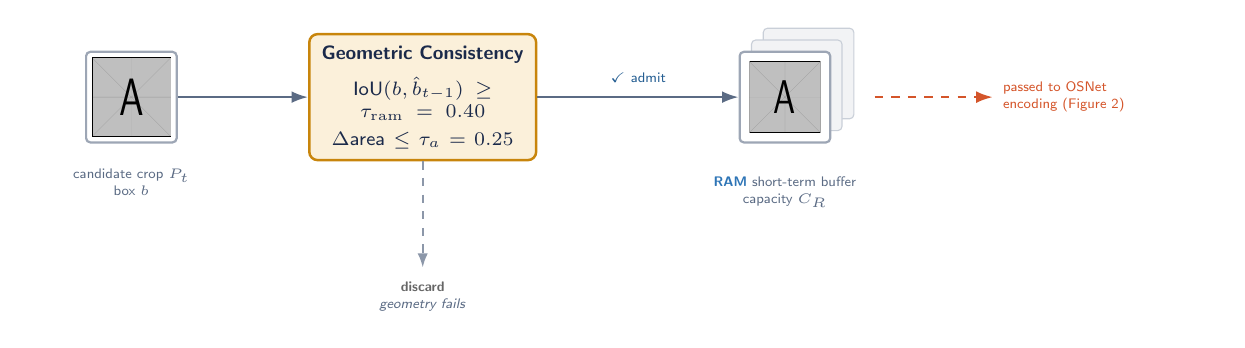
\begin{tikzpicture}[font=\small, x=1cm, y=1cm]

% ---------- main horizontal spine ----------
\node[imgcard] (patch) at (0,0) {\includegraphics[width=1.0cm,height=1.0cm]{example-image-a}};
\node[smallcaption, below=2mm of patch, text width=2.4cm]
      {candidate crop $P_t$\\ box $b$};

\node[gatebox] (gate) at (3.7,0) {%
  \textbf{Geometric Consistency}\\[4pt]
  {\scriptsize IoU$(b,\hat b_{t-1})\ge \tau_{\mathrm{ram}}=0.40$}\\[2pt]
  {\scriptsize $\Delta\text{area}\le \tau_{a}=0.25$}%
};

% ---------- RAM stack ----------
\node[ghostcard] (ramG2) at (8.60,0.30) {};
\node[ghostcard] (ramG1) at (8.45,0.15) {};
\node[imgcard]   (ramF)  at (8.30,0.00)
      {\includegraphics[width=0.9cm,height=0.9cm]{example-image-a}};
\node[smallcaption, below=3mm of ramF, text width=3.2cm]
      {\textbf{\textcolor{skyblue}{RAM}} short-term buffer\\ capacity $C_R$};

% ---------- arrows ----------
\draw[flow] (patch.east) -- (gate.west);
\draw[flow] (gate.east) -- node[above, font=\tiny, text=skyblue!80!black, yshift=0.5mm]
      {\checkmark~admit} (ramF.west);

% discard branch (label sits to the right of the arrow, not under it)
\draw[dashedflow] (gate.south) -- ++(0,-1.35)
      node[smallcaption, below=0.5mm, text width=2.8cm]
      {\textcolor{gray!80!black}{\textbf{discard}}\\ \textit{geometry fails}};

% exit stub -> Figure 2
\draw[flow, draw=coral, dashed] (ramF.east) ++(0.55,0) -- ++(1.5,0)
      node[right, font=\tiny, text=coral, align=left, text width=2.6cm]
      {passed to OSNet\\ encoding (Figure 2)};

\end{tikzpicture}%
}

\vspace{4mm}
\begin{center}
\begin{minipage}{0.86\textwidth}
\centering

\begin{tikzpicture}
\node[notebox, text width=0.95\textwidth] {%
  Only boxes that \textbf{stay put} and \textbf{stay the same size} enter RAM --- this blocks a
  same-frame distractor jump \emph{before} any identity check runs.};
\end{tikzpicture}
\end{minipage}
\end{center}

\end{frame}

% =====================================================
% FIGURE 2 : OSNet ENCODING + DRM (mathematical stacked matrix)
% =====================================================
\begin{frame}{Figure 2 --- OSNet Encoding \& the DRM Identity Matrix}

\centering
\resizebox{!}{0.86\textheight}{%
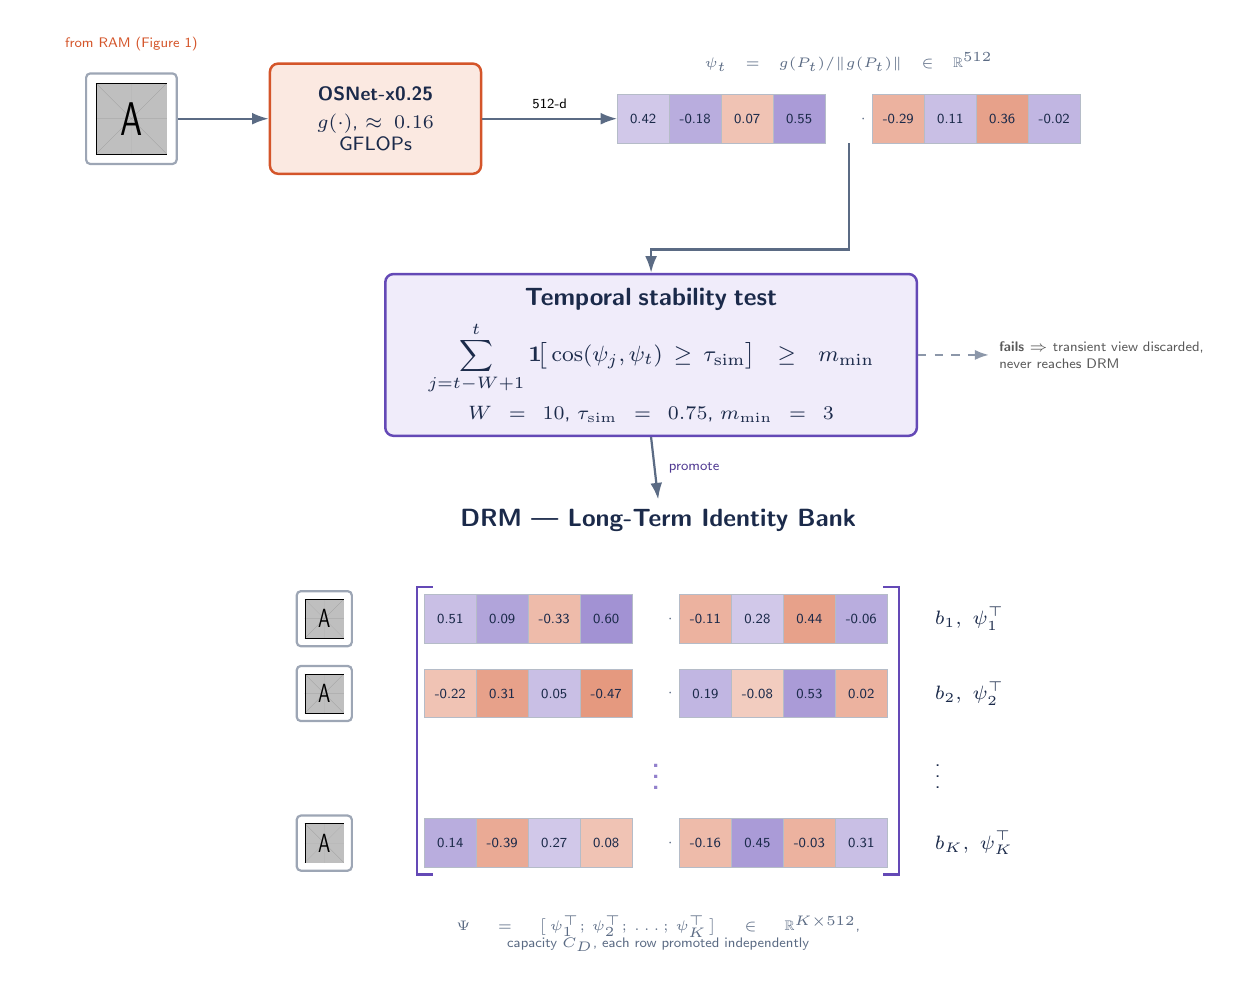
\begin{tikzpicture}[font=\small, x=1cm, y=1cm]

\def\rowspacing{0.95}
\def\cw{0.66}   % cell width in cm

% =========== STAGE 1 : encoding row (y = 0) ===========
\node[imgcard] (ramin) at (0,0) {\includegraphics[width=0.9cm,height=0.9cm]{example-image-a}};
\node[smallcaption, above=1.5mm of ramin, text width=2.4cm, text=coral]
      {from RAM (Figure 1)};

\node[procbox] (osnet) at (3.1,0) {\textbf{OSNet-x0.25}\\[2pt]{\scriptsize $g(\cdot)$, $\approx 0.16$ GFLOPs}};

\draw[flow] (ramin.east) -- (osnet.west);

% candidate embedding vector, first cell centred at x = 6.5
\begin{scope}[shift={(6.5,0)}]
  \foreach \i/\v/\c in {0/{0.42}/violet!30,1/{-0.18}/violet!45,2/{0.07}/coral!35,3/{0.55}/violet!55}{
    \node[numcell, fill=\c] at (\i*\cw,0) {\v};
  }
  \node[font=\tiny, text=slategray] at (4*\cw+0.3,0) {$\cdots$};
  \foreach \i/\v/\c in {0/{-0.29}/coral!45,1/{0.11}/violet!35,2/{0.36}/coral!55,3/{-0.02}/violet!40}{
    \node[numcell, fill=\c] at (4*\cw+0.6+\i*\cw,0) {\v};
  }
  \coordinate (vecLeft)   at (-0.33,0);
  \coordinate (vecBot)    at (3.5*\cw+0.3,-0.31);
  \node[smallcaption, text width=5.4cm] at (3.5*\cw+0.3,0.72)
        {$\psi_t = g(P_t)/\lVert g(P_t)\rVert \in \mathbb{R}^{512}$};
\end{scope}

\draw[flow] (osnet.east) -- node[above, font=\tiny]{512-d} (vecLeft);

% =========== STAGE 2 : temporal stability test ===========
\coordinate (spine) at (6.6,0);   % vertical spine x-coordinate

\node[eqbox] (eqbox) at (6.6,-3.00) {%
  \textbf{\small Temporal stability test}\\[3pt]
  {\footnotesize$\displaystyle\sum_{j=t-W+1}^{t}\mathbf{1}\!\big[\cos(\psi_j,\psi_t)\ge \tau_{\mathrm{sim}}\big] \;\ge\; m_{\min}$}\\[3pt]
  {\scriptsize $W=10$, $\tau_{\mathrm{sim}}=0.75$, $m_{\min}=3$}%
};

% orthogonal route: leaves the vector, steps left onto the spine, drops into the box
\draw[flow] (vecBot) -- ++(0,-1.35) -- (6.6,-1.66) -- (eqbox.north);

% failure branch exits sideways so it never fights the promote arrow
\draw[dashedflow] (eqbox.east) -- ++(0.9,0)
      node[right, font=\tiny, text=gray!70!black, align=left, text width=2.8cm]
      {\textbf{fails} $\Rightarrow$ transient view discarded, never reaches DRM};

% =========== STAGE 3 : DRM matrix ===========
\coordinate (matOrigin) at (4.05,-6.35);

\node[navy, font=\bfseries\small] (drmtitle) at (6.69,-5.10) {DRM --- Long-Term Identity Bank};

\draw[flow] (eqbox.south) -- node[right, font=\tiny, text=violet!80!black, xshift=0.5mm]{promote}
      (drmtitle.north);

% -- row 1 --
\begin{scope}[shift={(matOrigin)}]
  \node[imgcard, minimum width=7mm, minimum height=7mm] at (-1.6,0)
        {\includegraphics[width=5mm,height=5mm]{example-image-a}};
  \foreach \i/\v/\c in {0/{0.51}/violet!35,1/{0.09}/violet!50,2/{-0.33}/coral!40,3/{0.60}/violet!60}{
    \node[numcell, fill=\c] at (\i*\cw,0) {\v};
  }
  \node[font=\tiny, text=slategray] at (4*\cw+0.3,0) {$\cdots$};
  \foreach \i/\v/\c in {0/{-0.11}/coral!45,1/{0.28}/violet!30,2/{0.44}/coral!55,3/{-0.06}/violet!45}{
    \node[numcell, fill=\c] at (4*\cw+0.6+\i*\cw,0) {\v};
  }
  \node[font=\scriptsize, text=navy, anchor=west] at (8*\cw+0.75,0) {$b_1,\ \psi_1^{\top}$};
\end{scope}

% -- row 2 --
\begin{scope}[shift={($(matOrigin)+(0,-\rowspacing)$)}]
  \node[imgcard, minimum width=7mm, minimum height=7mm] at (-1.6,0)
        {\includegraphics[width=5mm,height=5mm]{example-image-a}};
  \foreach \i/\v/\c in {0/{-0.22}/coral!35,1/{0.31}/coral!55,2/{0.05}/violet!35,3/{-0.47}/coral!60}{
    \node[numcell, fill=\c] at (\i*\cw,0) {\v};
  }
  \node[font=\tiny, text=slategray] at (4*\cw+0.3,0) {$\cdots$};
  \foreach \i/\v/\c in {0/{0.19}/violet!40,1/{-0.08}/coral!30,2/{0.53}/violet!55,3/{0.02}/coral!45}{
    \node[numcell, fill=\c] at (4*\cw+0.6+\i*\cw,0) {\v};
  }
  \node[font=\scriptsize, text=navy, anchor=west] at (8*\cw+0.75,0) {$b_2,\ \psi_2^{\top}$};
\end{scope}

% -- ellipsis row --
\node[font=\Large, text=violet!70] at ($(matOrigin)+(3.5*\cw+0.3,-2*\rowspacing)$) {$\vdots$};
\node[font=\scriptsize, text=navy, anchor=west] at ($(matOrigin)+(8*\cw+0.75,-2*\rowspacing)$) {$\vdots$};

% -- row K --
\begin{scope}[shift={($(matOrigin)+(0,-3*\rowspacing)$)}]
  \node[imgcard, minimum width=7mm, minimum height=7mm] at (-1.6,0)
        {\includegraphics[width=5mm,height=5mm]{example-image-a}};
  \foreach \i/\v/\c in {0/{0.14}/violet!45,1/{-0.39}/coral!50,2/{0.27}/violet!30,3/{0.08}/coral!35}{
    \node[numcell, fill=\c] at (\i*\cw,0) {\v};
  }
  \node[font=\tiny, text=slategray] at (4*\cw+0.3,0) {$\cdots$};
  \foreach \i/\v/\c in {0/{-0.16}/coral!40,1/{0.45}/violet!55,2/{-0.03}/coral!45,3/{0.31}/violet!35}{
    \node[numcell, fill=\c] at (4*\cw+0.6+\i*\cw,0) {\v};
  }
  \node[font=\scriptsize, text=navy, anchor=west] at (8*\cw+0.75,0) {$b_K,\ \psi_K^{\top}$};
\end{scope}

% ---- big matrix brackets spanning all rows ----
\coordinate (bTL) at ($(matOrigin)+(-0.42, 0.40)$);
\coordinate (bBL) at ($(matOrigin)+(-0.42,-3*\rowspacing-0.40)$);
\coordinate (bTR) at ($(matOrigin)+(8*\cw+0.42, 0.40)$);
\coordinate (bBR) at ($(matOrigin)+(8*\cw+0.42,-3*\rowspacing-0.40)$);

\draw[line width=0.9pt, draw=violet] ($(bTL)+(0.2,0)$) -- (bTL) -- (bBL) -- ++(0.2,0);
\draw[line width=0.9pt, draw=violet] ($(bTR)+(-0.2,0)$) -- (bTR) -- (bBR) -- ++(-0.2,0);

\node[smallcaption, text width=8cm] at ($(matOrigin)+(2.64,-3*\rowspacing-1.15)$)
      {$\Psi = \big[\,\psi_1^{\top};\,\psi_2^{\top};\,\ldots;\,\psi_K^{\top}\,\big] \in \mathbb{R}^{K\times 512}$,\quad
       capacity $C_D$, each row promoted independently};

\end{tikzpicture}%
}

\end{frame}

% =====================================================
% FIGURE 2a : OSNet CONTRASTIVE (SIAMESE) TRAINING     [ADDED]
% =====================================================
\begin{frame}{Figure 2a --- Training OSNet by Contrastive (Siamese) Learning}

\centering
\vspace{-0.5mm}
\resizebox{!}{0.90\textheight}{%
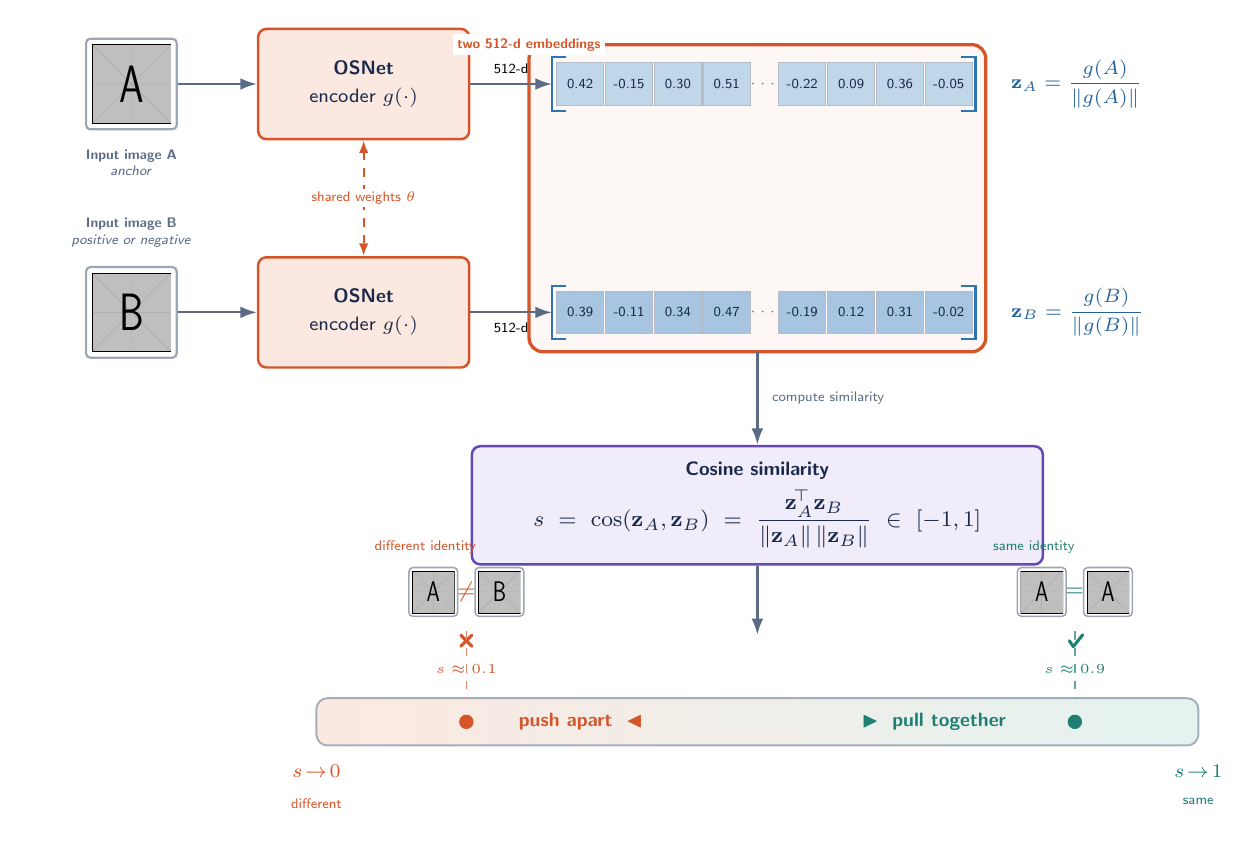
\begin{tikzpicture}[font=\small, x=1cm, y=1cm]

% ============================ TWIN BRANCHES ============================
% ---- top branch : anchor ----
\node[imgcard] (imgA) at (0,1.45)
      {\includegraphics[width=1.0cm,height=1.0cm]{example-image-a}};
\node[smallcaption, below=1.2mm of imgA, text width=2.2cm]
      {\textbf{Input image A}\\\textit{anchor}};
\node[procbox] (osA) at (2.95,1.45)
      {\textbf{OSNet}\\[2pt]{\scriptsize encoder $g(\cdot)$}};

% ---- bottom branch : positive / negative ----
\node[imgcard] (imgB) at (0,-1.45)
      {\includegraphics[width=1.0cm,height=1.0cm]{example-image-b}};
\node[smallcaption, above=1.2mm of imgB, text width=2.4cm]
      {\textbf{Input image B}\\\textit{positive or negative}};
\node[procbox] (osB) at (2.95,-1.45)
      {\textbf{OSNet}\\[2pt]{\scriptsize encoder $g(\cdot)$}};

\draw[flow] (imgA.east) -- (osA.west);
\draw[flow] (imgB.east) -- (osB.west);

% ---- shared weights tie ----
\draw[{Latex[length=1.6mm]}-{Latex[length=1.6mm]}, dashed, line width=0.8pt, draw=coral]
      (osA.south) -- (osB.north);
\node[font=\tiny, text=coral, fill=white, inner sep=1pt] at (2.95,0)
      {shared weights $\theta$};

% ============================ EMBEDDINGS + RED BOX =====================
% the RED box around the two embeddings (drawn first so cells sit on top)
\draw[coral, line width=1.2pt, rounded corners=5pt, fill=coral!4]
      (5.05,-1.95) rectangle (10.85,1.95);
\node[font=\tiny\bfseries, text=coral, fill=white, inner sep=1.5pt]
      at (5.05,1.95) {two 512-d embeddings};

% top embedding row z_A
\begin{scope}[shift={(5.7,1.45)}]
  \shrowN{skyblue!30}{0.42,-0.15,0.30,0.51,-0.22,0.09,0.36,-0.05}{}
  \sbracketsC{skyblue}{0.34}{-0.34}
\end{scope}
% bottom embedding row z_B
\begin{scope}[shift={(5.7,-1.45)}]
  \shrowN{skyblue!42}{0.39,-0.11,0.34,0.47,-0.19,0.12,0.31,-0.02}{}
  \sbracketsC{skyblue}{0.34}{-0.34}
\end{scope}

\draw[flow] (osA.east) -- node[above, font=\tiny]{512-d} (5.34,1.45);
\draw[flow] (osB.east) -- node[below, font=\tiny]{512-d} (5.34,-1.45);

% vector names (to the right, outside the box)
\node[font=\scriptsize, text=skyblue!85!black, anchor=west] at (11.05,1.45)
      {$\mathbf{z}_A=\dfrac{g(A)}{\lVert g(A)\rVert}$};
\node[font=\scriptsize, text=skyblue!85!black, anchor=west] at (11.05,-1.45)
      {$\mathbf{z}_B=\dfrac{g(B)}{\lVert g(B)\rVert}$};

% ============================ SIMILARITY ARROW ========================
\coordinate (boxbot) at (7.95,-1.95);
\node[eqbox, text width=6.9cm] (cos) at (7.95,-3.9)
   {\textbf{Cosine similarity}\\[3pt]
    {\footnotesize$\displaystyle s=\cos(\mathbf{z}_A,\mathbf{z}_B)
       =\frac{\mathbf{z}_A^{\!\top}\mathbf{z}_B}{\lVert\mathbf{z}_A\rVert\,\lVert\mathbf{z}_B\rVert}\in[-1,1]$}};
\draw[flow, line width=1.1pt] (boxbot) --
      node[right, font=\tiny, text=slategray, xshift=0.5mm]{compute similarity} (cos.north);

% ============================ SIMILARITY SCALE ========================
\def\barL{2.35} \def\barR{13.55} \def\barT{-6.35} \def\barB{-6.95}
\pgfmathsetmacro{\barW}{\barR-\barL}
\pgfmathsetmacro{\barC}{0.5*(\barT+\barB)}

\draw[flow, line width=1.1pt] (cos.south) -- (7.95,-5.55);

% the coral -> teal gradient track
\shade[left color=corallight, right color=tealmemlight, rounded corners=4pt]
      (\barL,\barB) rectangle (\barR,\barT);
\draw[rounded corners=4pt, draw=slategray!55, line width=0.7pt]
      (\barL,\barB) rectangle (\barR,\barT);

% end captions
\node[font=\scriptsize\bfseries, text=coral, anchor=north] at (\barL,\barB-0.12)
      {$s\!\to\!0$};
\node[smallcaption, text=coral, anchor=north] at (\barL,\barB-0.55) {different};
\node[font=\scriptsize\bfseries, text=tealmem, anchor=north] at (\barR,\barB-0.12)
      {$s\!\to\!1$};
\node[smallcaption, text=tealmem, anchor=north] at (\barR,\barB-0.55) {same};

% marker positions on the bar
\pgfmathsetmacro{\xNeg}{\barL+0.17*\barW}   % different pair
\pgfmathsetmacro{\xPos}{\barL+0.86*\barW}   % same pair

% direction labels sitting on the track
\node[font=\scriptsize\bfseries, text=coral]  at (\barL+0.30*\barW,\barC)
      {push apart $\;\blacktriangleleft$};
\node[font=\scriptsize\bfseries, text=tealmem] at (\barL+0.70*\barW,\barC)
      {$\blacktriangleright\;$ pull together};

% ---- NEGATIVE example (different identities) ----
\node[imgph] (nA) at (\xNeg-0.42,-5.0) {\includegraphics[width=0.54cm,height=0.54cm]{example-image-a}};
\node[imgph] (nB) at (\xNeg+0.42,-5.0) {\includegraphics[width=0.54cm,height=0.54cm]{example-image-b}};
\node[font=\footnotesize, text=coral] at (\xNeg,-5.0) {$\neq$};
\node[smallcaption, text=coral, above=0.5mm of nA.north east, xshift=-0.42cm]
      {different identity};
\nomark{\xNeg}{-5.62}
\node[font=\tiny\bfseries, text=coral, fill=white, inner sep=1pt] at (\xNeg,-5.98) {$s\approx0.1$};
\fill[coral] (\xNeg,\barC) circle (2.6pt);
\draw[coral!70, line width=0.6pt, dashed] (\xNeg,-5.5) -- (\xNeg,\barT);

% ---- POSITIVE example (same identity) ----
\node[imgph] (pA) at (\xPos-0.42,-5.0) {\includegraphics[width=0.54cm,height=0.54cm]{example-image-a}};
\node[imgph] (pB) at (\xPos+0.42,-5.0) {\includegraphics[width=0.54cm,height=0.54cm]{example-image-a}};
\node[font=\footnotesize, text=tealmem] at (\xPos,-5.0) {$=$};
\node[smallcaption, text=tealmem, above=0.5mm of pA.north east, xshift=-0.42cm]
      {same identity};
\okmark{\xPos}{-5.62}
\node[font=\tiny\bfseries, text=tealmem, fill=white, inner sep=1pt] at (\xPos,-5.98) {$s\approx0.9$};
\fill[tealmem] (\xPos,\barC) circle (2.6pt);
\draw[tealmem!70, line width=0.6pt, dashed] (\xPos,-5.5) -- (\xPos,\barT);

\end{tikzpicture}%
}

\vspace{1mm}
{\footnotesize The two crops pass through \emph{one} shared OSNet encoder. Training \textbf{pulls}
same-identity embeddings together ($s\!\to\!1$) and \textbf{pushes} different-identity ones apart
($s\!\to\!0$) --- the same cosine score later drives DRM matching at inference.}

\end{frame}

% =====================================================
% FIGURE 2b : DISTRACTOR-BANK CONSTRUCTION (sibling of Fig 2)  [ADDED]
% =====================================================
\begin{frame}{Figure 2b --- Distractor Bank: Red Detections $\to$ OSNet $\to$ Negative Matrix}

\centering
\resizebox{!}{0.86\textheight}{%
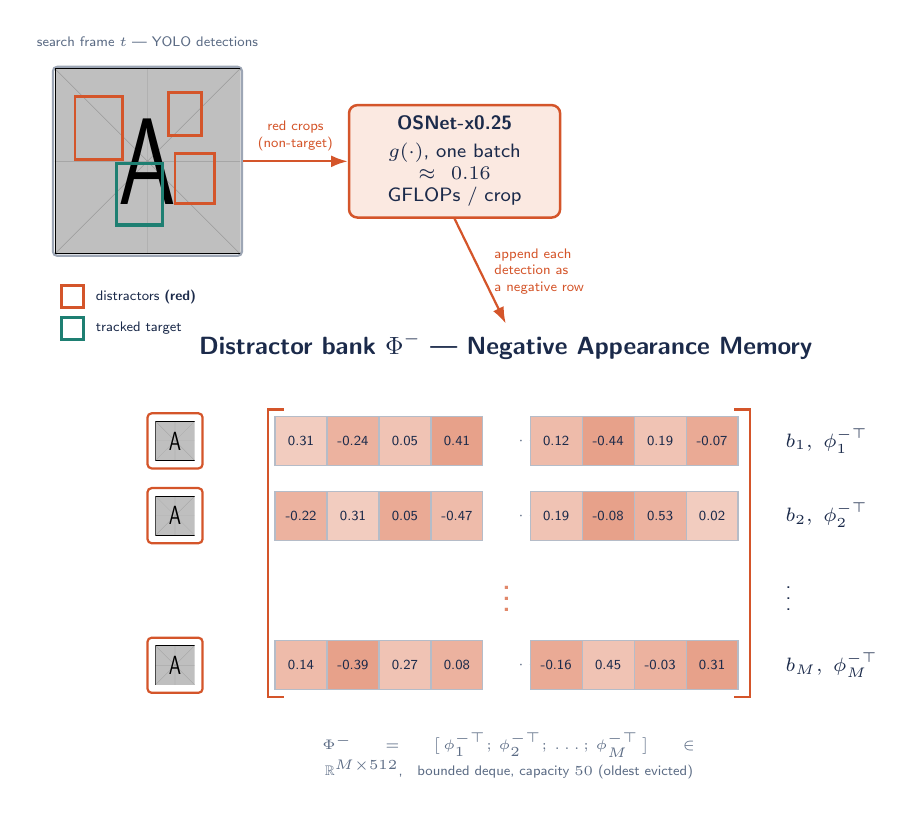
\begin{tikzpicture}[font=\small, x=1cm, y=1cm]

\def\rowspacing{0.95}
\def\cw{0.66}

% =========== STAGE 1 : annotated frame -> OSNet ===========
\node[imgcard, minimum width=2.4cm, minimum height=2.4cm] (frame) at (0,0)
      {\includegraphics[width=2.35cm,height=2.35cm]{example-image-a}};
\node[smallcaption, above=1.2mm of frame] {search frame $t$ --- YOLO detections};
% distractor detections (red)
\node[candbox, line width=1.0pt, minimum width=0.60cm, minimum height=0.80cm] at (-0.62,0.42) {};
\node[candbox, line width=1.0pt, minimum width=0.50cm, minimum height=0.64cm] at (0.60,-0.22) {};
\node[candbox, line width=1.0pt, minimum width=0.42cm, minimum height=0.54cm] at (0.48,0.60) {};
% tracked target (teal)
\node[gtbox, line width=1.2pt, minimum width=0.58cm, minimum height=0.78cm] at (-0.10,-0.42) {};
% legend
\node[candbox, line width=1.0pt, minimum width=0.28cm, minimum height=0.28cm] at (-0.95,-1.72) {};
\node[font=\tiny, text=navy, anchor=west] at (-0.78,-1.72) {distractors \textbf{(red)}};
\node[gtbox, line width=1.2pt, minimum width=0.28cm, minimum height=0.28cm] at (-0.95,-2.12) {};
\node[font=\tiny, text=navy, anchor=west] at (-0.78,-2.12) {tracked target};

\node[procbox] (osnet) at (3.9,0) {\textbf{OSNet-x0.25}\\[2pt]{\scriptsize $g(\cdot)$, one batch}\\{\scriptsize $\approx0.16$ GFLOPs / crop}};
\draw[flow, draw=coral] (frame.east) --
      node[above, font=\tiny, text=coral, align=center]{red crops\\ (non-target)} (osnet.west);

% =========== STAGE 2 : route into the bank ===========
\coordinate (matOrigin) at (1.95,-3.55);
\node[navy, font=\bfseries\small] (banktitle) at (4.55,-2.35)
      {Distractor bank $\Phi^{-}$ --- Negative Appearance Memory};
\draw[flow, draw=coral] (osnet.south) -- node[right, font=\tiny, text=coral, xshift=0.5mm, align=left]
      {append each\\ detection as\\ a negative row} (banktitle.north);

% =========== STAGE 3 : the stacked negative matrix ===========
% -- row 1 --
\begin{scope}[shift={(matOrigin)}]
  \node[imgcard, draw=coral, minimum width=7mm, minimum height=7mm] at (-1.6,0)
        {\includegraphics[width=5mm,height=5mm]{example-image-a}};
  \foreach \i/\v/\c in {0/{0.31}/coral!30,1/{-0.24}/coral!45,2/{0.05}/coral!35,3/{0.41}/coral!55}{
    \node[numcell, fill=\c] at (\i*\cw,0) {\v};}
  \node[font=\tiny, text=slategray] at (4*\cw+0.3,0) {$\cdots$};
  \foreach \i/\v/\c in {0/{0.12}/coral!40,1/{-0.44}/coral!55,2/{0.19}/coral!35,3/{-0.07}/coral!50}{
    \node[numcell, fill=\c] at (4*\cw+0.6+\i*\cw,0) {\v};}
  \node[font=\scriptsize, text=navy, anchor=west] at (8*\cw+0.75,0) {$b_1,\ \phi_1^{-\top}$};
\end{scope}
% -- row 2 --
\begin{scope}[shift={($(matOrigin)+(0,-\rowspacing)$)}]
  \node[imgcard, draw=coral, minimum width=7mm, minimum height=7mm] at (-1.6,0)
        {\includegraphics[width=5mm,height=5mm]{example-image-a}};
  \foreach \i/\v/\c in {0/{-0.22}/coral!45,1/{0.31}/coral!30,2/{0.05}/coral!50,3/{-0.47}/coral!40}{
    \node[numcell, fill=\c] at (\i*\cw,0) {\v};}
  \node[font=\tiny, text=slategray] at (4*\cw+0.3,0) {$\cdots$};
  \foreach \i/\v/\c in {0/{0.19}/coral!35,1/{-0.08}/coral!55,2/{0.53}/coral!45,3/{0.02}/coral!30}{
    \node[numcell, fill=\c] at (4*\cw+0.6+\i*\cw,0) {\v};}
  \node[font=\scriptsize, text=navy, anchor=west] at (8*\cw+0.75,0) {$b_2,\ \phi_2^{-\top}$};
\end{scope}
% -- ellipsis row --
\node[font=\Large, text=coral!70] at ($(matOrigin)+(3.5*\cw+0.3,-2*\rowspacing)$) {$\vdots$};
\node[font=\scriptsize, text=navy, anchor=west] at ($(matOrigin)+(8*\cw+0.75,-2*\rowspacing)$) {$\vdots$};
% -- row M --
\begin{scope}[shift={($(matOrigin)+(0,-3*\rowspacing)$)}]
  \node[imgcard, draw=coral, minimum width=7mm, minimum height=7mm] at (-1.6,0)
        {\includegraphics[width=5mm,height=5mm]{example-image-a}};
  \foreach \i/\v/\c in {0/{0.14}/coral!40,1/{-0.39}/coral!55,2/{0.27}/coral!35,3/{0.08}/coral!45}{
    \node[numcell, fill=\c] at (\i*\cw,0) {\v};}
  \node[font=\tiny, text=slategray] at (4*\cw+0.3,0) {$\cdots$};
  \foreach \i/\v/\c in {0/{-0.16}/coral!50,1/{0.45}/coral!35,2/{-0.03}/coral!45,3/{0.31}/coral!55}{
    \node[numcell, fill=\c] at (4*\cw+0.6+\i*\cw,0) {\v};}
  \node[font=\scriptsize, text=navy, anchor=west] at (8*\cw+0.75,0) {$b_M,\ \phi_M^{-\top}$};
\end{scope}

% ---- big matrix brackets spanning all rows ----
\coordinate (bTL) at ($(matOrigin)+(-0.42, 0.40)$);
\coordinate (bBL) at ($(matOrigin)+(-0.42,-3*\rowspacing-0.40)$);
\coordinate (bTR) at ($(matOrigin)+(8*\cw+0.42, 0.40)$);
\coordinate (bBR) at ($(matOrigin)+(8*\cw+0.42,-3*\rowspacing-0.40)$);
\draw[line width=0.9pt, draw=coral] ($(bTL)+(0.2,0)$) -- (bTL) -- (bBL) -- ++(0.2,0);
\draw[line width=0.9pt, draw=coral] ($(bTR)+(-0.2,0)$) -- (bTR) -- (bBR) -- ++(-0.2,0);

\node[smallcaption, text width=8.4cm] at ($(matOrigin)+(2.64,-3*\rowspacing-1.15)$)
      {$\Phi^{-}=\big[\,\phi_1^{-\top};\,\phi_2^{-\top};\,\ldots;\,\phi_M^{-\top}\,\big]\in\mathbb{R}^{M\times512}$,\quad
       bounded deque, capacity $50$ (oldest evicted)};

\end{tikzpicture}%
}

\end{frame}

% =====================================================
% FIGURE 3 : EKF -- WHERE to search
% =====================================================
\begin{frame}{Figure 3 --- EKF: \emph{Where} to Search (Camera-Aware Prediction)}

\centering
\vspace{1mm}
\resizebox{0.96\textwidth}{!}{%
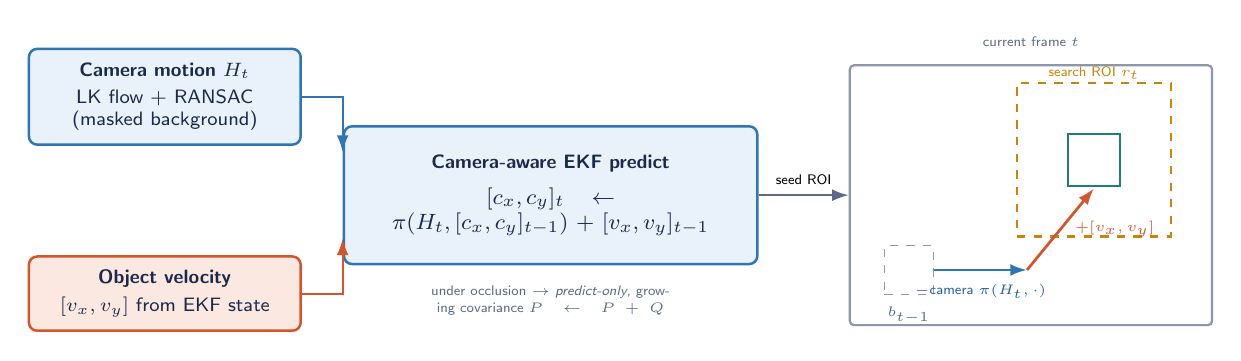
\begin{tikzpicture}[font=\small, x=1cm, y=1cm]

% ---- inputs (stacked left) ----
\node[ekfbox, text width=3.1cm] (cam) at (0,1.25)
   {\textbf{Camera motion} $H_t$\\[2pt]{\scriptsize LK flow $+$ RANSAC\\(masked background)}};
\node[ekfbox, text width=3.1cm, draw=coral, fill=corallight] (vel) at (0,-1.25)
   {\textbf{Object velocity}\\[2pt]{\scriptsize $[v_x,v_y]$ from EKF state}};

% ---- EKF predict (center) : one equation, detail moved to a tag below ----
\node[ekfbox, text width=4.9cm, minimum height=1.75cm] (ekf) at (4.9,0)
   {\textbf{Camera-aware EKF predict}\\[5pt]
    {\footnotesize$[c_x,c_y]_t \leftarrow \pi(H_t,[c_x,c_y]_{t-1}) + [v_x,v_y]_{t-1}$}};
\node[smallcaption, text width=4.7cm, text=slategray, below=1.4mm of ekf]
   {under occlusion $\rightarrow$ \emph{predict-only}, growing covariance $P\leftarrow P+Q$};

\draw[flow, draw=skyblue] (cam.east) -| ($(ekf.west)+(0,0.55)$);
\draw[flow, draw=coral]   (vel.east) -| ($(ekf.west)+(0,-0.55)$);

% ---- result frame (right) : clean two-step dogleg ----
\begin{scope}[shift={(11.0,0)}]
  \node[framecard, minimum width=4.6cm, minimum height=3.3cm] (fr) at (0,0) {};
  \node[smallcaption, above=1mm of fr] {current frame $t$};

  % previous box (ghost) -> waypoint (camera slide removed) -> predicted box
  \node[draw=slategray!70, dashed, minimum width=0.62cm, minimum height=0.62cm] (old) at (-1.55,-0.95) {};
  \node[smallcaption, below=0.3mm of old] {$b_{t-1}$};
  \coordinate (warp) at (-0.05,-0.95);
  \node[gtbox, minimum width=0.66cm, minimum height=0.66cm] (pred) at (0.80,0.45) {};

  % ROI around predicted
  \node[roi, minimum width=1.95cm, minimum height=1.95cm] (roibox) at (0.80,0.45) {};
  \node[smallcaption, text=amber] at (0.80,1.55) {search ROI $r_t$};

  % step 1: subtract camera slide (horizontal), step 2: add object velocity (up)
  \draw[flow, draw=skyblue, line width=1pt] (old.east) -- (warp)
        node[midway, below=0.5mm, font=\tiny, text=skyblue!85!black]{$-$camera $\pi(H_t,\cdot)$};
  \draw[flow, draw=coral, line width=1pt] (warp) -- ($(pred.south)+(0,-0.02)$)
        node[midway, right=0.5mm, font=\tiny, text=coral]{$+[v_x,v_y]$};
\end{scope}

\draw[flow] (ekf.east) -- node[above,font=\tiny]{seed ROI} (fr.west);

\end{tikzpicture}}

\vspace{3mm}
\begin{center}\begin{minipage}{0.9\textwidth}\centering
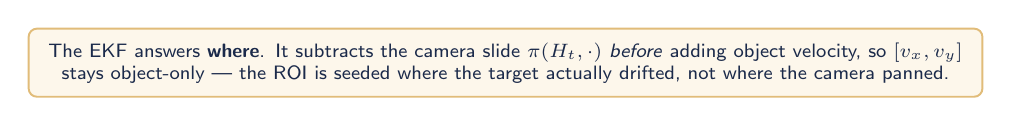
\begin{tikzpicture}\node[notebox, text width=0.97\textwidth]{%
The EKF answers \textbf{where}. It subtracts the camera slide $\pi(H_t,\cdot)$ \emph{before} adding object
velocity, so $[v_x,v_y]$ stays object-only --- the ROI is seeded where the target actually drifted, not
where the camera panned.};\end{tikzpicture}
\end{minipage}\end{center}

\end{frame}

% =====================================================
% FIGURE 4 : YOLO on the ROI -> candidates
% =====================================================
\begin{frame}{Figure 4 --- YOLO on the ROI: Proposing Candidates}

\centering
\vspace{1mm}
\resizebox{0.96\textwidth}{!}{%
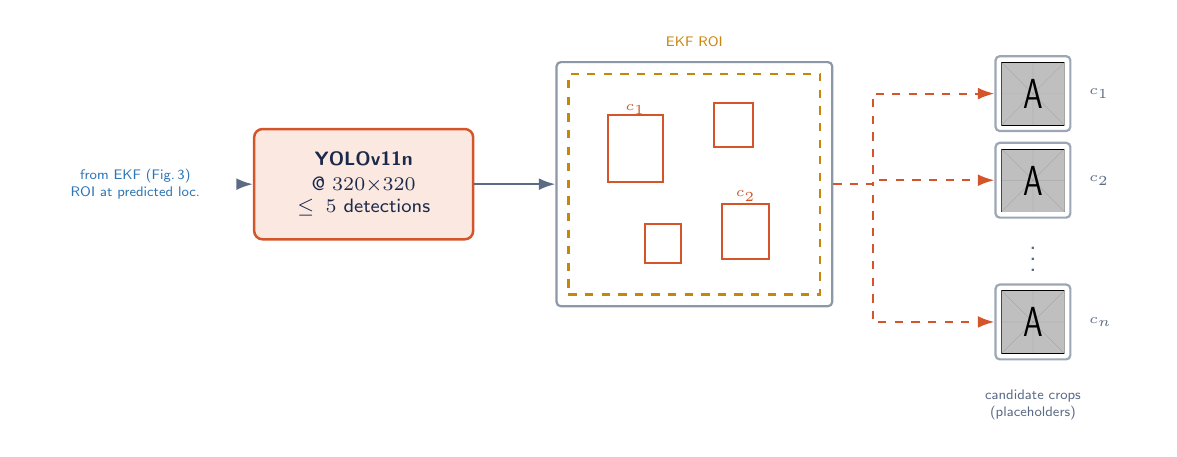
\begin{tikzpicture}[font=\small, x=1cm, y=1cm]

% source
\node[smallcaption, text width=2.5cm, text=skyblue] (src) at (0,0)
   {from EKF (Fig.\,3)\\ ROI at predicted loc.};
\node[procbox, text width=2.5cm] (yolo) at (2.9,0)
   {\textbf{YOLOv11n}\\[1pt]{\scriptsize @ $320{\times}320$}\\{\scriptsize $\le 5$ detections}};
\draw[flow] (src.east) -- (yolo.west);

% ROI picture with candidate boxes drawn inside
\begin{scope}[shift={(7.1,0)}]
  \node[framecard, minimum width=3.5cm, minimum height=3.1cm] (roi) at (0,0) {};
  \node[roi, minimum width=3.2cm, minimum height=2.8cm] at (0,0) {};
  \node[smallcaption, text=amber, above=0.6mm of roi] {EKF ROI};
  \node[candbox, minimum width=0.7cm, minimum height=0.85cm] at (-0.75,0.45) {};
  \node[font=\tiny,text=coral] at (-0.75,0.95){$c_1$};
  \node[candbox, minimum width=0.6cm, minimum height=0.7cm] at (0.65,-0.6) {};
  \node[font=\tiny,text=coral] at (0.65,-0.15){$c_2$};
  \node[candbox, minimum width=0.5cm, minimum height=0.55cm] at (0.5,0.75) {};
  \node[candbox, minimum width=0.45cm, minimum height=0.5cm] at (-0.4,-0.75) {};
\end{scope}
\draw[flow] (yolo.east) -- (roi.west);

% extracted candidate crops
\begin{scope}[shift={(11.4,0)}]
  \node[cropcard] (cr1) at (0,1.15) {\includegraphics[width=0.8cm,height=0.8cm]{example-image-a}};
  \node[cropcard] (cr2) at (0,0.05) {\includegraphics[width=0.8cm,height=0.8cm]{example-image-a}};
  \node[font=\normalsize, text=slategray] at (0,-0.85) {$\vdots$};
  \node[cropcard] (crn) at (0,-1.75) {\includegraphics[width=0.8cm,height=0.8cm]{example-image-a}};
  \node[smallcaption, right=1mm of cr1]{$c_1$};
  \node[smallcaption, right=1mm of cr2]{$c_2$};
  \node[smallcaption, right=1mm of crn]{$c_n$};
  \node[smallcaption, text width=2.7cm, below=2.5mm of crn]{candidate crops\\(placeholders)};
\end{scope}
\draw[flow, draw=coral, dashed] (roi.east) -- ++(0.5,0) |- (cr1.west);
\draw[flow, draw=coral, dashed] (roi.east) -- ++(0.5,0) |- (cr2.west);
\draw[flow, draw=coral, dashed] (roi.east) -- ++(0.5,0) |- (crn.west);

\end{tikzpicture}}

\vspace{3mm}
\begin{center}\begin{minipage}{0.9\textwidth}\centering
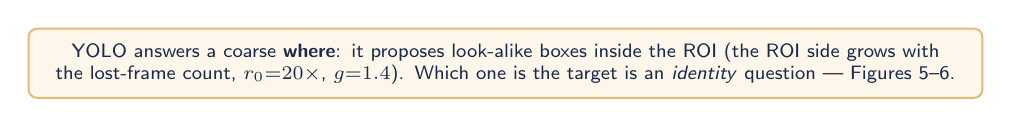
\begin{tikzpicture}\node[notebox, text width=0.97\textwidth]{%
YOLO answers a coarse \textbf{where}: it proposes look-alike boxes inside the ROI (the ROI side grows
with the lost-frame count, $r_0{=}20{\times}$, $g{=}1.4$). Which one is the target is an \emph{identity}
question --- Figures 5--6.};\end{tikzpicture}
\end{minipage}\end{center}

\end{frame}

% =====================================================
% FIGURE 5 : candidates -> OSNet -> embedding matrix
% =====================================================
\begin{frame}{Figure 5 --- Encoding Candidates: One OSNet Batch}

\centering
\vspace{2mm}
\resizebox{0.97\textwidth}{!}{%
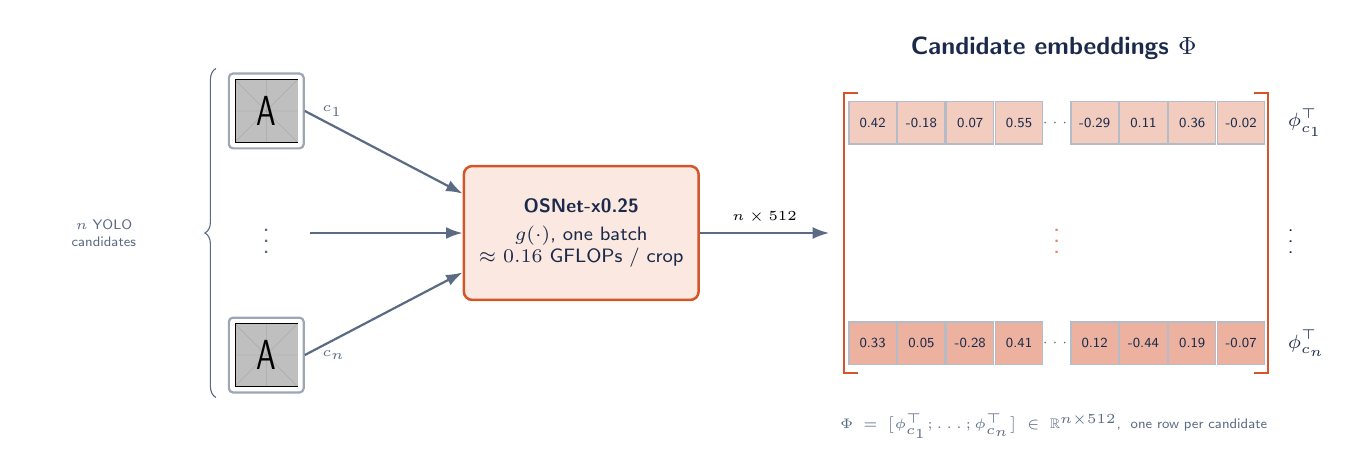
\begin{tikzpicture}[font=\small, x=1cm, y=1cm]

% ---- candidate crops (top c_1, dots, bottom c_n) ----
\node[cropcard] (c1) at (0,1.55) {\includegraphics[width=0.8cm,height=0.8cm]{example-image-a}};
\node[smallcaption, right=1mm of c1]{$c_1$};
\node[font=\normalsize, text=slategray] at (0,0.0) {$\vdots$};
\node[cropcard] (cn) at (0,-1.55) {\includegraphics[width=0.8cm,height=0.8cm]{example-image-a}};
\node[smallcaption, right=1mm of cn]{$c_n$};

% brace on the LEFT (arrows exit right, so no crossing)
\draw[decorate, decoration={brace, amplitude=4pt, mirror}, draw=slategray]
      ($(c1.north west)+(-0.15,0.05)$) -- ($(cn.south west)+(-0.15,-0.05)$);
\node[smallcaption, text width=1.7cm, left=6mm of c1, yshift=-1.55cm]{$n$ YOLO\\candidates};

% ---- OSNet ----
\node[procbox, text width=2.7cm, minimum height=1.7cm] (osnet) at (4.0,0)
   {\textbf{OSNet-x0.25}\\[2pt]{\scriptsize $g(\cdot)$, one batch}\\{\scriptsize $\approx0.16$ GFLOPs / crop}};
\draw[flow] (c1.east) -- ($(osnet.west)+(0,0.5)$);
\draw[flow] (0.55,0) -- ($(osnet.west)+(0,0)$);
\draw[flow] (cn.east) -- ($(osnet.west)+(0,-0.5)$);

% ---- candidate embedding matrix Phi ----
\begin{scope}[shift={(7.7,0)}]
  \begin{scope}[shift={(0,1.4)}]
    \shrowN{coral!30}{0.42,-0.18,0.07,0.55,-0.29,0.11,0.36,-0.02}{$\phi_{c_1}^{\top}$};
  \end{scope}
  \node[font=\normalsize, text=coral!70] at (4*\cwS-0.14,0.0) {$\vdots$};
  \node[font=\scriptsize, text=navy, anchor=west] at (5.15,0.0){$\vdots$};
  \begin{scope}[shift={(0,-1.4)}]
    \shrowN{coral!45}{0.33,0.05,-0.28,0.41,0.12,-0.44,0.19,-0.07}{$\phi_{c_n}^{\top}$};
  \end{scope}
  \sbracketsC{coral}{1.78}{-1.78}
  \node[navy, font=\bfseries\small] at (2.3,2.35) {Candidate embeddings $\Phi$};
  \node[smallcaption, text width=6cm] at (2.3,-2.45)
     {$\Phi=\big[\phi_{c_1}^{\top};\ldots;\phi_{c_n}^{\top}\big]\in\mathbb{R}^{n\times512}$,\ \ one row per candidate};
\end{scope}
\draw[flow] (osnet.east) -- node[above,font=\tiny]{$n\times512$} (7.7-0.55,0);

\end{tikzpicture}}

\vspace{2mm}
{\footnotesize All candidate crops are L2-normalised and encoded in \emph{one} OSNet pass, yielding a
candidate embedding matrix $\Phi$ --- ready to compare against the identity bank.}

\end{frame}

% =====================================================
% FIGURE 6 : DRM comparison + acceptance
% =====================================================
\begin{frame}{Figure 6 --- \emph{Which}: DRM Match, Margin, and Tracker Confirm}

\centering
\vspace{-1mm}
\resizebox{0.99\textwidth}{!}{%
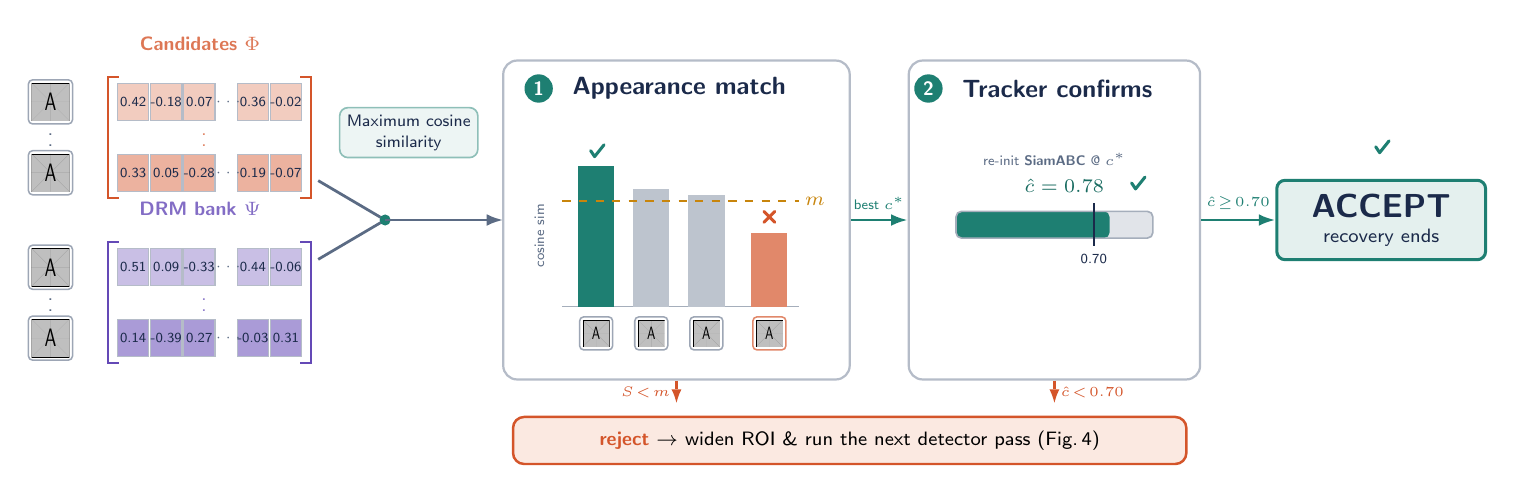
\begin{tikzpicture}[font=\small, x=1cm, y=1cm,
   panel/.style={rounded corners=5pt, draw=slategray!45, line width=0.8pt, fill=white},
   ttlchip/.style={circle, draw=none, fill=tealmem, text=white, font=\bfseries\scriptsize,
                   inner sep=0pt, minimum size=3.6mm},
   retrybar/.style={rounded corners=4pt, draw=coral, line width=0.9pt, fill=corallight,
                    font=\scriptsize, align=center, inner sep=5pt, text width=8.2cm},
   imgph/.style={draw=slategray!60, line width=0.55pt, rounded corners=1.5pt, fill=white,
                    inner sep=0pt, minimum width=0.56cm, minimum height=0.56cm}]

% ================= TWO VECTORS (each row = one crop + its embedding) =================
\begin{scope}[shift={(0.35,1.55)}]
  \node[coral!80, font=\bfseries\scriptsize] at (0.85,0.74) {Candidates $\Phi$};
  % row 1 crop  -- replace example-image-a with your candidate image
  \node[imgph] at (-1.05,0.0)  {\includegraphics[width=0.48cm,height=0.48cm]{example-image-a}};
  \begin{scope}[shift={(0,0.0)}]  \shrowK{coral!30}{0.42,-0.18,0.07,0.36,-0.02}{} \end{scope}
  % continuation
  \node[font=\scriptsize, text=slategray] at (-1.05,-0.45) {$\vdots$};
  \node[font=\scriptsize, text=coral!70]  at (0.90,-0.45) {$\vdots$};
  % row n crop  -- replace example-image-a with your candidate image
  \node[imgph] at (-1.05,-0.9) {\includegraphics[width=0.48cm,height=0.48cm]{example-image-a}};
  \begin{scope}[shift={(0,-0.9)}] \shrowK{coral!45}{0.33,0.05,-0.28,0.19,-0.07}{} \end{scope}
  \sbracketsK{coral}{0.32}{-1.22}
\end{scope}

\begin{scope}[shift={(0.35,-0.55)}]
  \node[violet!80, font=\bfseries\scriptsize] at (0.85,0.74) {DRM bank $\Psi$};
  % memory slot 1 crop  -- replace example-image-a with your memory image
  \node[imgph] at (-1.05,0.0)  {\includegraphics[width=0.48cm,height=0.48cm]{example-image-a}};
  \begin{scope}[shift={(0,0.0)}]  \shrowK{violet!35}{0.51,0.09,-0.33,0.44,-0.06}{} \end{scope}
  % continuation
  \node[font=\scriptsize, text=slategray] at (-1.05,-0.45) {$\vdots$};
  \node[font=\scriptsize, text=violet!70] at (0.90,-0.45) {$\vdots$};
  % memory slot K crop  -- replace example-image-a with your memory image
  \node[imgph] at (-1.05,-0.9) {\includegraphics[width=0.48cm,height=0.48cm]{example-image-a}};
  \begin{scope}[shift={(0,-0.9)}] \shrowK{violet!55}{0.14,-0.39,0.27,-0.03,0.31}{} \end{scope}
  \sbracketsK{violet}{0.32}{-1.22}
\end{scope}

% ===== combine both vectors: maximum cosine similarity =====
\coordinate (mrg) at (3.55,0.05);
\draw[line width=1pt, draw=slategray] (2.70,0.55)  -- (mrg);   % candidates in
\draw[line width=1pt, draw=slategray] (2.70,-0.45) -- (mrg);   % memory in
\fill[tealmem] (mrg) circle (2pt);
\draw[flow, line width=1pt, draw=slategray] (mrg) -- (5.05,0.05);   % out to panel 1
\node[rounded corners=3pt, fill=tealmem!8, draw=tealmem!50, line width=0.6pt,
      inner sep=2.6pt, align=center, font=\fontsize{6.5}{7.5}\selectfont, text=navy]
      at (3.85,1.16) {Maximum cosine\\similarity};

% ================= PANEL 1 : APPEARANCE MATCH (bar chart) =================
\node[panel, minimum width=4.4cm, minimum height=4.05cm] (p1) at (7.25,0.05) {};
\node[ttlchip] (t1) at (5.50,1.72) {1};
\node[right=1.2mm of t1, font=\bfseries\small, text=navy] {Appearance match};

\begin{scope}[shift={(5.85,-1.05)}]  % chart origin (baseline-left)
  \draw[slategray!55, line width=0.6pt] (-0.05,0) -- (2.95,0);           % baseline
  % bars
  \fill[tealmem]      (0.15,0) rectangle (0.61,1.78);
  \fill[slategray!40] (0.85,0) rectangle (1.31,1.50);
  \fill[slategray!40] (1.55,0) rectangle (2.01,1.42);
  \fill[coral!70]     (2.35,0) rectangle (2.81,0.94);
  % threshold line m
  \draw[amber, line width=0.9pt, dashed] (-0.05,1.34) -- (2.95,1.34);
  \node[amber, font=\scriptsize] at (3.16,1.34) {$m$};
  % pass / fail glyphs
  \okmark{0.38}{1.98}
  \nomark{2.58}{1.14}
  % candidate crop thumbnails under each bar  -- replace example-image-a with your crops
  \node[imgph, minimum width=0.42cm, minimum height=0.42cm]
        at (0.38,-0.34) {\includegraphics[width=0.34cm,height=0.34cm]{example-image-a}};
  \node[imgph, minimum width=0.42cm, minimum height=0.42cm]
        at (1.08,-0.34) {\includegraphics[width=0.34cm,height=0.34cm]{example-image-a}};
  \node[imgph, minimum width=0.42cm, minimum height=0.42cm]
        at (1.78,-0.34) {\includegraphics[width=0.34cm,height=0.34cm]{example-image-a}};
  \node[imgph, minimum width=0.42cm, minimum height=0.42cm, draw=coral!70]
        at (2.58,-0.34) {\includegraphics[width=0.34cm,height=0.34cm]{example-image-a}};
  \node[font=\tiny, text=slategray, rotate=90] at (-0.34,0.9) {cosine sim};
\end{scope}

% ================= PANEL 2 : TRACKER CONFIRMS (gauge) =================
\node[panel, minimum width=3.7cm, minimum height=4.05cm] (p2) at (12.05,0.05) {};
\node[ttlchip] (t2) at (10.45,1.72) {2};
\node[right=1.2mm of t2, font=\bfseries\small, text=navy] {Tracker confirms};

\node[font=\tiny, text=slategray, align=center] at (12.05,0.82)
     {re-init \textbf{SiamABC} @ $c^{*}$};

\begin{scope}[shift={(10.80,-0.18)}]   % gauge origin (track-left)
  \def\gW{2.5}
  \fill[slategray!18, rounded corners=2pt] (0,0) rectangle (\gW,0.34);
  \fill[tealmem, rounded corners=2pt]      (0,0) rectangle (0.78*\gW,0.34);
  \draw[slategray!55, rounded corners=2pt, line width=0.6pt] (0,0) rectangle (\gW,0.34);
  % threshold at 0.70
  \draw[navy, line width=0.8pt] (0.70*\gW,-0.10) -- (0.70*\gW,0.44);
  \node[font=\fontsize{5}{5}\selectfont, text=navy] at (0.70*\gW,-0.26) {0.70};
  % current value + pass
  \node[font=\scriptsize, text=tealmem!85!black] at (0.55*\gW,0.66) {$\hat c=0.78$};
  \okmark{2.30}{0.70}
\end{scope}

% ================= ACCEPT =================
\okmark{16.20}{0.98}
\node[acceptbox, text width=2.3cm, minimum height=1.0cm] (accept) at (16.20,0.05)
     {\large ACCEPT\\[1pt]\normalsize\mdseries\scriptsize recovery ends};

% ================= FLOW BETWEEN CHECKPOINTS =================
\draw[flow, draw=tealmem, line width=1pt] (p1.east) --
      node[above, font=\tiny, text=tealmem]{best $c^{*}$} (p2.west);
\draw[flow, draw=tealmem, line width=1pt] (p2.east) --
      node[above, font=\tiny, text=tealmem]{$\hat c\!\ge\!0.70$} (accept.west);

% ================= RETRY (either check fails) =================
\node[retrybar] (retry) at (9.45,-2.75)
     {\textbf{\textcolor{coral}{reject}} $\rightarrow$ widen ROI \& run the next detector pass (Fig.\,4)};
\draw[dashedflow, draw=coral] (p1.south) --
      node[left, font=\tiny, text=coral, xshift=0.5mm]{$S\!<\!m$} (7.25,-2.28);
\draw[dashedflow, draw=coral] (p2.south) --
      node[right, font=\tiny, text=coral, xshift=-0.5mm]{$\hat c\!<\!0.70$} (12.05,-2.28);

\end{tikzpicture}}

\vspace{1.2mm}
{\footnotesize \textbf{Two independent checks, both required.} A look-alike in the right place still
scores low on identity; the resuming tracker's own confidence $\hat c$ seals it --- one lucky false
detection cannot hijack the track.}

\end{frame}

% =====================================================
% FIGURE 6b : DISTRACTOR-AWARE SCORING (subtraction hint)  [ADDED]
% =====================================================
\begin{frame}{Figure 6b --- Distractor-Aware Scoring: Subtract the Distractor Match}

\centering
\vspace{1mm}
\resizebox{0.99\textwidth}{!}{%
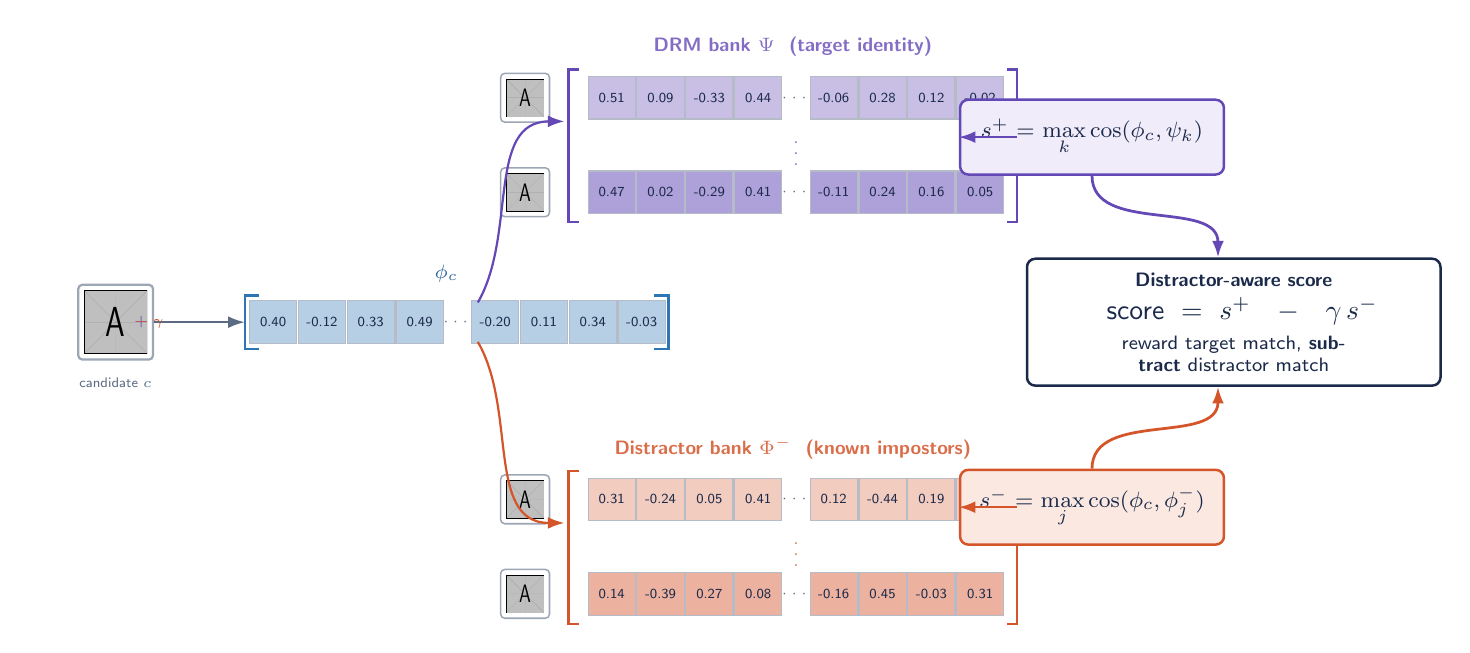
\begin{tikzpicture}[font=\small, x=1cm, y=1cm]

% ---- candidate embedding (center-left) ----
\node[cropcard] (cc) at (0,0) {\includegraphics[width=0.8cm,height=0.8cm]{example-image-a}};
\node[smallcaption, below=1mm of cc, text width=2.0cm]{candidate $c$};
\begin{scope}[shift={(2.0,0)}]
  \shrowN{skyblue!35}{0.40,-0.12,0.33,0.49,-0.20,0.11,0.34,-0.03}{}
  \sbracketsC{skyblue}{0.34}{-0.34}
\end{scope}
\node[font=\scriptsize, text=skyblue!85!black] at (4.2,0.62) {$\phi_c$};
\draw[flow] (cc.east) -- (1.64,0);

% ================= TOP branch : DRM target bank (reward) =================
\begin{scope}[shift={(6.3,2.55)}]
  \node[violet!80, font=\bfseries\scriptsize] at (2.3,0.95) {DRM bank $\Psi$ \ (target identity)};
  \begin{scope}[shift={(0,0.30)}]
    \node[imgph] at (-1.1,0){\includegraphics[width=0.48cm,height=0.48cm]{example-image-a}};
    \shrowN{violet!35}{0.51,0.09,-0.33,0.44,-0.06,0.28,0.12,-0.02}{}
  \end{scope}
  \node[font=\scriptsize, text=violet!70] at (4*\cwS-0.14,-0.30){$\vdots$};
  \begin{scope}[shift={(0,-0.90)}]
    \node[imgph] at (-1.1,0){\includegraphics[width=0.48cm,height=0.48cm]{example-image-a}};
    \shrowN{violet!52}{0.47,0.02,-0.29,0.41,-0.11,0.24,0.16,0.05}{}
  \end{scope}
  \draw[line width=0.8pt, draw=violet] (-0.42,0.66) -- (-0.55,0.66) -- (-0.55,-1.28) -- (-0.42,-1.28);
  \draw[line width=0.8pt, draw=violet] (5.02,0.66) -- (5.15,0.66) -- (5.15,-1.28) -- (5.02,-1.28);
\end{scope}
\node[eqbox, draw=violet, fill=violetlight, text width=3.0cm, minimum height=0.95cm] (splus)
      at (12.4,2.35)
      {\footnotesize$s^{+}=\displaystyle\max_{k}\cos(\phi_c,\psi_k)$};
\draw[flow, draw=violet] (4.6,0.25) to[out=60,in=180] (6.3-0.6,2.55);
\draw[flow, draw=violet] (6.3+5.15,2.35) -- (splus.west);

% ================= BOTTOM branch : distractor bank (penalty) =================
\begin{scope}[shift={(6.3,-2.55)}]
  \node[coral!85, font=\bfseries\scriptsize] at (2.3,0.95) {Distractor bank $\Phi^{-}$ \ (known impostors)};
  \begin{scope}[shift={(0,0.30)}]
    \node[imgph] at (-1.1,0){\includegraphics[width=0.48cm,height=0.48cm]{example-image-a}};
    \shrowN{coral!30}{0.31,-0.24,0.05,0.41,0.12,-0.44,0.19,-0.07}{}
  \end{scope}
  \node[font=\scriptsize, text=coral!70] at (4*\cwS-0.14,-0.30){$\vdots$};
  \begin{scope}[shift={(0,-0.90)}]
    \node[imgph] at (-1.1,0){\includegraphics[width=0.48cm,height=0.48cm]{example-image-a}};
    \shrowN{coral!45}{0.14,-0.39,0.27,0.08,-0.16,0.45,-0.03,0.31}{}
  \end{scope}
  \draw[line width=0.8pt, draw=coral] (-0.42,0.66) -- (-0.55,0.66) -- (-0.55,-1.28) -- (-0.42,-1.28);
  \draw[line width=0.8pt, draw=coral] (5.02,0.66) -- (5.15,0.66) -- (5.15,-1.28) -- (5.02,-1.28);
\end{scope}
\node[eqbox, draw=coral, fill=corallight, text width=3.0cm, minimum height=0.95cm] (sminus)
      at (12.4,-2.35)
      {\footnotesize$s^{-}=\displaystyle\max_{j}\cos(\phi_c,\phi^{-}_{j})$};
\draw[flow, draw=coral] (4.6,-0.25) to[out=-60,in=180] (6.3-0.6,-2.55);
\draw[flow, draw=coral] (6.3+5.15,-2.35) -- (sminus.west);

% ================= COMBINE : score = s+ - gamma s- =================
\node[eqbox, text width=4.9cm, minimum height=1.55cm, draw=navy, fill=white] (score) at (14.2,0)
      {\textbf{Distractor-aware score}\\[4pt]
       {\normalsize$\;\text{score}=s^{+}\;-\;\gamma\, s^{-}$}\\[3pt]
       {\scriptsize reward target match, \textbf{subtract} distractor match}};
\draw[flow, draw=violet, line width=1pt] (splus.south) to[out=-90,in=90] ($(score.north)+(-0.2,0)$)
      node[midway, right=1mm, font=\tiny, text=violet]{$+$};
\draw[flow, draw=coral, line width=1pt] (sminus.north) to[out=90,in=-90] ($(score.south)+(-0.2,0)$)
      node[midway, right=1mm, font=\tiny, text=coral]{$-\,\gamma$};

\end{tikzpicture}%
}

\vspace{2mm}
\begin{center}\begin{minipage}{0.92\textwidth}\centering

\begin{tikzpicture}\node[notebox, text width=0.97\textwidth]{%
A look-alike in the right place still scores high on the target bank $s^{+}$ --- but if it also matches a
\textbf{banked distractor} it earns a large $s^{-}$, and $-\gamma s^{-}$ \textbf{pulls its score back down}.
Only a candidate that matches the target \emph{and} none of the known impostors survives.};\end{tikzpicture}
\end{minipage}\end{center}

\end{frame}

\end{document}
